\documentclass[9pt]{beamer}

\ifluatex 
  \usepackage{fontspec}
\else\ifxetex
  \usepackage{fontspec}
\else
  \usepackage[utf8]{inputenc}
  \usepackage[T2A,T1]{fontenc}
  \usepackage{textcomp}
\fi\fi 

\usepackage{booktabs}
\usepackage{tabularx} 

\title{Conception de profileurs non intrusifs pour le faisceau de protons de ESS}
\author{Florian Benedetti}
\institute{CEA/IRFU}
\date{23/09/2019}

\usetheme[]{Frankfurt}
\usecolortheme{beaver}

\setbeamerfont{title}{size=\Huge}
\setbeamerfont{frametitle}{size=\huge}

\AtBeginSection[]{
 \begin{frame}
 \vfill
 \centering
 \begin{beamercolorbox}[sep=8pt,center,shadow=true,rounded=true]{title}
   \usebeamerfont{title}\insertsectionhead\par%
 \end{beamercolorbox}
 \vfill
 \tableofcontents[sectionstyle=show/hide,subsectionstyle=show/show/hide]{}

 %\tableofcontents[currentsubsection]
 \end{frame}
}

\setbeamertemplate{footline}%{infolines theme}
{
  \leavevmode%
  \hbox{%
  \begin{beamercolorbox}[wd=.25\paperwidth,ht=2.25ex,dp=1ex,center]   {author in head/foot}%
    \usebeamerfont{author in head/foot}\insertshortauthor
  \end{beamercolorbox}%
  \begin{beamercolorbox}[wd=.50\paperwidth,ht=2.25ex,dp=1ex,center]{title in head/foot}%
   \usebeamerfont{title in head/foot}\insertshorttitle
  \end{beamercolorbox}%
  \begin{beamercolorbox}[wd=.25\paperwidth,ht=2.25ex,dp=1ex,right]{date in head/foot}%
    \insertframenumber{} / \inserttotalframenumber\hspace*{2ex} 
  \end{beamercolorbox}}%
 \vskip0pt%
}

\newcommand{\backupbegin}{
   \newcounter{finalframe}
   \setcounter{finalframe}{\value{framenumber}}
}
\newcommand{\backupend}{
   \setcounter{framenumber}{\value{finalframe}}
}


\begin{document}
\frame{\titlepage}

\begin{frame}
  \frametitle{Presentation outline}
  \tableofcontents[subsectionstyle=hide/hide/hide]
\end{frame}


\section{Introduction}
\begin{frame}
  \frametitle{Context}
  \begin{columns}
    \begin{column}{0.45\textwidth}
      \begin{block}{Neutron}
        \begin{itemize}
          \item Neutral particle
          \item Wave–particle duality
          \item Magnetic moment
        \end{itemize}
      \end{block}
    \end{column}
    \begin{column}{0.45\textwidth}
      \begin{block}{As probe}
        \begin{itemize}
          \item High penetration
          \item Large scale
          \item 
        \end{itemize}
      \end{block}
    \end{column}
  \end{columns}
  \includegraphics[width=\textwidth]{01_Neutron/fig/fig000_Dague.png}
\end{frame}

\subsection{Context}
\begin{frame}
  \frametitle{State of Neutron sources}
  \begin{block}{Producing neutron}
    Producing neutron is not a trivial task
  \end{block}
  \begin{columns}
    \begin{column}{0.45\textwidth}
      \begin{block}{Fission reactor}
        Use fission reaction:
        \begin{equation*}
          _{92}^{235}U + n \rightarrow X + Y + k \times n
        \end{equation*}
        Continuous flux
      \end{block}
    \end{column}
    \begin{column}{0.45\textwidth}
      \begin{block}{Accelerator Driven Source}
        Two methods:
        \begin{itemize}
          \item
          \item Spallation: with dense target ()
        \end{itemize}
        The properties of theses sources strongly depends on the accelerator.
      \end{block}
    \end{column}
  \end{columns}
  \begin{block}{Spallation}
    Spallation is efficient : a single particle/target collision can generate more than 20 neutrons ...
  \end{block}
\end{frame}

\begin{frame}
  \frametitle{State of Neutron sources}
  \begin{columns}
    \begin{column}{0.50\textwidth}
      \includegraphics[width=\textwidth]{01_Neutron/fig/fig000_NeutronSources_a}
    \end{column}
    \begin{column}{0.50\textwidth}
      \includegraphics[width=\textwidth]{01_Neutron/fig/fig000_NeutronSources_b}
    \end{column}
  \end{columns}
  From "Neutron scattering facilities in Europe" report by ESFRI
\end{frame}

\subsection{European Spallation Source}
\begin{frame}
  \frametitle{European Spallation Source}
  \begin{block}{Mandate}
    ESS will be the next high end European neutron source.

    Based on a 2 GeV proton accelerator and a tungsten target
  \end{block}
  \begin{columns}
    \begin{column}{0.4\textwidth}
      \begin{block}{Key points}
        \begin{itemize}
          \item[2014] Ground breacking
          \item[2021] First protons on target
          \item[2023] Beginning of user program
          \item 15 neutron instruments
          \item Total cost: 1.8 B€
        \end{itemize}
      \end{block}
    \end{column}
    \begin{column}{0.65\textwidth}
      \includegraphics[width=\textwidth]{01_Neutron/fig/fig000_ESS_pulse.jpeg}
    \end{column}
  \end{columns}
\end{frame}

\begin{frame}
  \frametitle{The accelerator}
  \includegraphics[width=\textwidth]{01_Neutron/fig/fig000_ESS_acc}
  \vfill
  \begin{columns}
    \begin{column}{0.45\textwidth}
      \begin{block}{Key points}
        The accelerator itself is a big challenge.
        \begin{itemize}
          \item 600 m long with 356 m of acceleration
          \item d
          \item 95.5
        \end{itemize}
      \end{block}
    \end{column}
    \begin{column}{0.50\textwidth}
      \begin{tabularx}{\linewidth}{XX}
        \toprule
        Characteristic & Value                                 \\
        \midrule
        Energy         & $2\,\mathrm{GeV}$                     \\
        Current        & $62.5\,\mathrm{mA}$                   \\
        Duration       & $2.86\,\mathrm{ms}$                   \\
        Rep. rate      & $14\,\mathrm{Hz}$                     \\
        Duty cycle     & $4\,\mathrm{\%}$                      \\
        Power (peak)   & $5\,\mathrm{MW}$ ($125\,\mathrm{MW}$) \\
        RF             & $352.21\,\mathrm{MHz}$                \\
                       & $704.42\,\mathrm{MHz}$                \\
        \bottomrule
      \end{tabularx}
    \end{column}
  \end{columns}
\end{frame}
\section{Beam diagnostic and IPM}
\subsection{Beam diagnostic at ESS}
\begin{frame}
  \frametitle{Beam diagnostic at ESS}
  \begin{block}{ESS is based on a power accelerator}
    Beam diagnostics are mandatory tools to insure safety and acquire knowledge about the beam:
    \begin{itemize}
      \item 15 different systems: Beam position, beam current, beam energy, beam losses ...
      \item A total of 480 beam diagnostics along the accelerator.
      \item Various fields are involved in the development of these devices.
    \end{itemize}
  \end{block}

  Today, we are presenting a device that measure the \textbf{transverse beam profile}:
  \begin{columns}
    \begin{column}{0.60\textwidth}
      \begin{block}{Definition}
        Spacial distribution of the charges of the beam in the transverse plane.
        \begin{itemize}
          \item Beam shape
          \item Beam position
          \item Relative beam amplitude
        \end{itemize}
      \end{block}
    \end{column}
    \begin{column}{0.30\textwidth}
      \centering
      \includegraphics[width=0.5\textwidth]{02_ESS/fig/fig000_profile2}
    \end{column}
  \end{columns}
\end{frame}

% \begin{frame}
%   \frametitle{Profile measurement method}
%   \includegraphics[width=\textwidth]{01_Neutron/fig/fig000_ESS_acc}
%   \begin{columns}
%     \begin{column}{0.45\textwidth}
%       \begin{block}{Wire Scanner/SEM Grid}
%         Measurement of the secondaries electrons or hadronic cascade emitted during the collision of proton with one or more wires.
%       \end{block}
%       \begin{block}{Pros/cons}
%         \begin{itemize}
%           \item[+] High sensitivity
%           \item[-] Interceptive measurement
%         \end{itemize}
%       \end{block}
%     \end{column}
%     \begin{column}{0.45\textwidth}
%       Image/Schema
%       \begin{block}{Use at ESS}
%         \begin{itemize}
%           \item Everywhere along accelerator
%           \item But limited to low duty cycle
%         \end{itemize}
%       \end{block}
%     \end{column}
%   \end{columns}
%   \begin{alertblock}{Wire scanners cannot work at nominal conditions}
%     The WS can not withstand the $5\,\mathrm{MW}$ beam power. Wire can melt and may compromise the SC cavities.
%   \end{alertblock}
% \end{frame}

\subsection{Profile measurement method at ESS}
\begin{frame}
  \frametitle{Profile measurement method}
  \includegraphics[width=\textwidth]{01_Neutron/fig/fig000_ESS_acc}
  \begin{columns}
    \begin{column}{0.45\textwidth}
      \begin{block}{Fluorescence \textbf{Profile Monitor} (FPM)}
        Measurement of the fluorescence induced by the beam.
      \end{block}
      \begin{block}{Pros/cons}
        \begin{itemize}
          \item[+] Non-invasive
          \item[+] No active elements in vacuum
          \item[-] $4\pi$ solid angle
          \item[-] Depends on vacuum
        \end{itemize}
      \end{block}
    \end{column}
    \begin{column}{0.45\textwidth}
      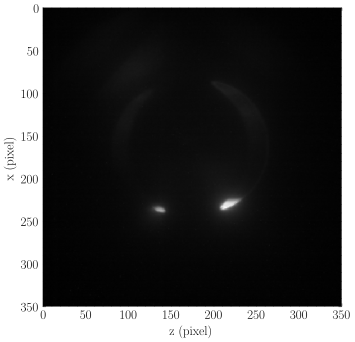
\includegraphics[width=\textwidth]{02_ESS/fig/fig000_FPM}

      \begin{block}{Use at ESS}
        \begin{itemize}
          \item In the warm parts of the accelerator
        \end{itemize}
      \end{block}
    \end{column}
  \end{columns}
  \begin{alertblock}{FPM cannot work in superconducing part}
    In the cryogenic section, the pressure is too low for FPM (expected $10^{-9}\,\mathrm{mbar}$).
  \end{alertblock}
\end{frame}

\begin{frame}
  \frametitle{Ionization Profile Monitor}
  \begin{alertblock}{So no profile measurement in SC part at nominal condition?}
    The measurement can be done by using an Ionization \textbf{Profile Monitor} (IPM).
  \end{alertblock}

  \begin{columns}
    \begin{column}{0.45\textwidth}
      \begin{block}{How it works}
        \begin{enumerate}
          \item Beam protons pass through the residual gas, inducing ionizations: $e^-$/ion pairs.
          \item An electric field drives $e^-$ or ions towards a segmented readout system.
          \item Profile in one transverse direction. Complete profile: pair of IPMs.
        \end{enumerate}
      \end{block}
    \end{column}
    \begin{column}{0.45\textwidth}
      \centering
      \includegraphics[width=0.8\textwidth]{02_ESS/fig/fig000_IPM.pdf}
    \end{column}
  \end{columns}
\end{frame}

\begin{frame}
  \frametitle{IPM}
  \begin{columns}[T]
    \begin{column}{0.45\textwidth}
      \begin{block}{Pros/cons}
        \begin{itemize}
          \item[+] Direct collection
          \item[+] Non invasive method
          \item[-] Vacuum dependant
          \item[-] Complex and expansive design (frame, HV, readout in vacuum)
          \item[-] Profile distortion
        \end{itemize}
      \end{block}

    \end{column}
    \begin{column}{0.45\textwidth}
      \begin{block}{History}
        \begin{itemize}
          \item 1960-1970: First use of an IPM.
          \item 1990-2000: Development of MCPs.
          \item 2015: Interest in semiconductor (CERN).
          \item Improvement of electronics and simulation capabilities.
        \end{itemize}
      \end{block}
    \end{column}
  \end{columns}


  IPMs are popular on proton circular accelerators or storage rings:
  \begin{itemize}
    \item Where vacuum can be extremely low (below $10^{-10}\,\mathrm{mbar}$)
    \item Pulse passes several times in the IPM
  \end{itemize}
  IPMs become popular for high intensity superconducting LINAC.
\end{frame}

\subsection{Project overview}
\begin{frame}
  \frametitle{Project overview}
  \begin{alertblock}{Subject of the thesis:}
    \textbf{Can we use IPMs in the superconducting part of the ESS accelerator?}
  \end{alertblock}
  \begin{block}{Project in brief}
    Provide 5 pairs of IPMs for the superconducting part of the ESS accelerator.

    Project milestones:
    \begin{itemize}
      \item[2016] Kick-off meeting (April), beginning of my PhD (October)
      \item[2017] Preliminary Design Review (February), \textbf{simulations, design and manufacturing}
      \item[2018] \textbf{Mainly beam tests and data analysis}
      \item[2019] Critical Design Review (March), design and manufacturing of final IPMs, end of my PhD (October)
      \item[2020] First IPM delivery, Handover
    \end{itemize}
  \end{block}
\end{frame}
\chapter{Prototype simulations and desing}
\chaptermark{Prototype simulations and desing}
\cleardoublepage[]
\minitoc[]
\section{Introduction}
\begin{refsection}
	\label{ch3:Introduction}
	First the requirements for will be
	Then
	Lastly
	\section{Taille de la page}
	textwidth in cm: \printinunitsof{cm}\prntlen{\textwidth}
	\section{ESS requirements}
	\input{03_Prototype/figures/00_fig/figure009_IPM_outline.tex}

	\begin{figure}[ht]
	\includegraphics[width=\textwidth]{03_Prototype/figures/00_fig/fig007_LWU.jpeg}
	\caption[Typical mass stopping power plot]{Typical mass stopping power plot.}
	\label{chap3:maxwell_gas_log1}
\end{figure}

	\section{Electromagnetic fields simulations}

	\begin{align}
		 & \overrightarrow{\nabla} \cdot \overrightarrow{E} = \frac{\rho}{\epsilon_{0}}                                            \\
		 & \overrightarrow{\nabla} \times \overrightarrow{E} = - \frac{\partial \overrightarrow{B}}{\partial t}                    \\
		 & \overrightarrow{\nabla} \cdot \overrightarrow{B} = 0                                                                    \\
		 & \overrightarrow{\nabla} \times \overrightarrow{B} = \overrightarrow{J} + \frac{\partial \overrightarrow{E}}{\partial t}
	\end{align}

	\section{Extraction field}
	\subsection{Maxwell equations at steady state}
	\subsection{Solving poisson equation}

	\begin{align}
		 & f(x+h) = f(x)+hf^{\prime}(x)
		+\frac{h^2}{2}f^{\prime\prime}(x)+\frac{h^3}{6}f^{\prime\prime\prime}(x) + O(h^{4}) \\
		 & f(x-h) = f(x)-hf^{\prime}(x)
		+\frac{h^2}{2}f^{\prime\prime}(x)-\frac{h^3}{6}f^{\prime\prime\prime}(x) + O(h^{4})
	\end{align}

	\begin{equation}
		f^{\prime\prime}(x) = \frac{f(x+h) + f(x-h) - 2f(x)}{h^{2}} + O(h^{2})
	\end{equation}

	\begin{equation}
		\begin{split}
			h^{2}f^{\prime\prime}(x,y)=&f(x+h,y) + f(x-h,y) \\
			+ &f(x,y+h) + f(x,y-h) \\
			- 4&f(x)+ O(h^{2})
		\end{split}
	\end{equation}

	%\subsection{Finite Elements Method}
	\subsection{COMSOL}
	COMSOL\cite{comsol2018} is a proprietary software.\cite{comsolacdc2018}

	\begin{figure}[ht]
	\includegraphics[width=\textwidth]{03_Prototype/figures/00_fig/fig003_COMSOL_LWU.jpeg}
	\caption[]{}
	\label{chap3:COMSOL_LWU}
\end{figure}


	\begin{figure}[ht]
	\includegraphics[width=\textwidth]{03_Prototype/figures/00_fig/fig006_COMSOL_meshing_elements.png}
	\caption[3D Mesh elements included in COMSOL]{Mesh elements included in COMSOL software. COMSOL uses tetrahedral elements by default to mesh a 3D geometry.}
	\label{chap3:maxwell_gas_log1}
\end{figure}


	\cite{cststudio2018}\cite{ansys2018}\cite{couloumb2018}
	\subsection{Criteria}
	\begin{figure}[ht]
	\includesvg[width=\textwidth]{03_Prototype/figures/00_fig/figure008_lorentz_evsp}
	\caption[Typical mass stopping power plot]{Typical mass stopping power plot.}
	\label{chap3:maxwell_gas_log1}
\end{figure}


	\subsection{IPM geometry}
	\subsection{IPM position and cross interaction}
	\subsection{Grid}
	\subsection{Field corrections}
	\subsection{IPM polarity}
	\section{Particle through matter}
	%TODO: Finir
	The interactions of particles with matter are an important aspect of nuclear or particle detection\cite[]{Leo1994, Knoll2010}.
	A particle loses energy when it passes through a medium.
	The physical process behind the energy transfer mainly depends on the characteristics of the particle.
	These topics has been studied and improved over the last century.
	It often combines complicated theoretical laws with approximations or empirical models.
	This topic is very wide, hence only the meaningful processes that are related to the IPMs will be described in the following sections.

	\subsection{Interraction of heavy charged particles with matter}
	%TODO: Finir
	For heavy charged particles, the main interaction is due to electromagnetic interactions of the incident particle with the orbiting electrons of the medium.
	A particle is considered heavy if its mass is far higher than the mass of an electron.
	The incident particle will transfer its energy to an electron of the medium at each electronic collision.
	The maximum transfer energy for one collision is given by the following equation:
	\begin{equation}
		T_{max} = \frac{2 m_{e} \beta^{2} \gamma^{2}}{1 + \frac{2 \gamma m_{e} }{M} + \left( \frac{m_{e}}{M} \right)^{2}}
	\end{equation}
	Where \(M\) is the mass of the incident particle and \(m_{e}\) is the mass of electron.

	The average linear stopping power is given equation\cite[]{Bethe1930} \cite[p. 446]{Tanabashi2018}
	\begin{equation}
		- \bigg \langle \frac{dE}{dx} \bigg \rangle =K \rho \frac{Z}{A} \frac{z^{2}}{\beta^{2}} \left[\frac{1}{2} ln \left(\frac{2 m_{e} \beta^{2} \gamma^{2} T_{max}}{I^{2}} \right) - \beta^{2} - \frac{\delta(\beta \gamma)}{2} - \frac{C}{Z} \right]
	\end{equation}
	The K constant is completely independant to the incident particle or the medium.

	Terms related to the medium, \(Z\) atomic number, \(A\) mass number, \(I\) mean excitation energy and \(\rho \) the medium density.
	One can see that the ratio \(Z/A\) is around \(0.5\) except for an hydrogen medium.

	The terms related to the incident particle with \(\gamma\) \(\beta\) \(z\)

	Nevertheless the Bethe equation still quite precise for particle between

	The Fig. \ref{chap3:bethe1} shows

	\begin{figure}[ht]
	\includesvg[width=\textwidth]{03_Prototype/figures/00_fig/fig001_bethe_2}
	\caption[Typical mass stopping power plot for protons]{Typical mass stopping power plot for protons. Here the mass stopping is plotted for proton in hydrogen and nitrogen.The calculation was done with respect to the Bethe formula and has been crosschecked with NIST PSTAR table which contains both computed and experimental values \cite{Seltzer1993}. The Bethe equation gives between \(0.2\ <\ \beta\gamma\ <\ 100\). However at lower and higher energies the Bethe formula is no more reliable.}
	\label{chap3:bethe1}
\end{figure}


	\subsection{Interraction of light charged particles in matter}
	%TODO: Finish
	If the incident particle
	In case of the incident particle is an electron the
	So the Bethe Bloch should be corrected for electron.\cite{Rieke1972}
	\begin{equation}
		- \bigg \langle \frac{dE}{dx} \bigg \rangle = \frac{1}{2} K \rho \frac{Z}{A} \frac{1}{\beta^{2}} \left[ln \left(\frac{2 m_{e} \beta^{2} \gamma^{2}}{2I^{2}} \right) + (1 - \beta^{2})\right]
	\end{equation}

	\subsection{Silicon based readout}
	\begin{figure}[ht]
	\includesvg[width=\textwidth]{03_Prototype/figures/00_fig/fig004_ion_si_deposit}
	\caption[Typical mass stopping power plot]{Typical mass stopping power plot.}
	\label{chap3:bethe1}
\end{figure}

	\begin{figure}[ht]
	\includesvg[width=\textwidth]{03_Prototype/figures/00_fig/fig005_ion_si_range}
	\caption[Typical mass stopping power plot]{Typical mass stopping power plot.}
	\label{chap3:bethe1}
\end{figure}


	\subsection{Electron ion pairs production}
	%TODO: Finish
	The mean linear stopping power.

	\cite[]{Weiss1955}
	\cite[]{Bichsel1979}
	\begin{equation}
		N_{electrons}= \frac{\big \langle \frac{dE}{dx} \big \rangle}{W_{n}} dx
	\end{equation}

	\begin{table}[ht]
	\centering
	\caption[W values for severals gases]
	{W values for severals gases.}
	\label{}
	\begin{tabular}{llr}
		\toprule
		Gas       & Description & Price (\$) \\
		\midrule
		Gnat      & per gram    & 13.65      \\
		          & each        & 0.01       \\
		Gnu       & stuffed     & 92.50      \\
		Emu       & stuffed     & 33.33      \\
		Armadillo & frozen      & 8.99       \\
		\bottomrule
	\end{tabular}
\end{table}

	The W value is usually measured

	\subsection{Case of a mixture}
	%TODO: Finish
	When the medium is a mixture of several compounds then it is necessary to calculate the mean stopping power for each of them with respect to their mass proportions:
	\begin{equation}
		N_{total}= \sum_{n= First}^{Last} N_{compound\ n}= \sum_{n= First}^{Last} w_{n} \frac{\big \langle \frac{dE}{dx}\left(\rho_{n},I_{n},A_{n},Z_{n}\right) \big \rangle}{W_{n}} dx
	\end{equation}
	The calculation can be done for each single element or for each molecule in the compound.
	However the second computation is preferable since the \(I\) and \(W\) values are in general smaller for mo.
	\subsection{Calculation}
	\begin{table}[ht]
	\centering
	\caption[Expected residual vacuum gas characteristics in the cold part of the ESS Linac, provided by ESS vacuum group]
	{Expected residual vacuum gas characteristics in the cold part of the ESS Linac, provided by ESS vacuum group.}
	\label{chap3:ess_vacuum_gas}
	\begin{tabular}{llll}
		\toprule
		Gas        & Mass percentage (\(\%)\) & $p_{i}$ (\(\mathrm{mbar}\)) & $\rho_{i}$ $(\mathrm{g/cm^{3}}$) \\
		\midrule
		\(H_{2}\)  & \(79\)                   & \(7.9\cdot10^{-10}\)        & \(6.52\cdot
		10^{-17}\)                                                                                             \\
		\(CO\)     & \(10\)                   & \(1.0\cdot10^{-10}\)        & \(1.15\cdot
		10^{-16}\)                                                                                             \\
		\(CO_{2}\) & \(10\)                   & \(1.0\cdot10^{-10}\)        & \(1.80\cdot
		10^{-16}\)                                                                                             \\
		\(N_{2}\)  & \(1\)                    & \(1.0\cdot10^{-11}\)        & \(1.14\cdot
		10^{-17}\)                                                                                             \\
		\bottomrule
	\end{tabular}
\end{table}
	\subsection{Simulations}
	\subsection{Limits}
	\subsection{Initial momentum}
	\begin{figure}[ht]
	\includesvg[width=\textwidth]{03_Prototype/figures/00_fig/fig002_maxwell_gas_log}
	\caption[Typical mass stopping power plot]{Typical mass stopping power plot.}
	\label{chap3:maxwell_gas_log1}
\end{figure}

	\section{Readout simulations}
	\subsection{Ramo-Schoktley theorem}
	\cite[]{Ramo_1939}\cite[]{Shockley_1938}\cite[]{Cavalleri1971}\cite[]{Jen1941}
	\subsection{Strips based readout}
	\subsection{MCP based readout}
	\subsubsection{Micro Channel Plate}
	\subsubsection{MCP models}
	\subsubsection{TimePix3}
	\subsubsection{Simulations}
	\subsubsection{Tests at IRMA}

	\section{Summary}
	\label{ch3:Summary}

	\cleardoublepage
	\section{Bibliography}
	\label{ch3:bib}
	\printbibliography[heading=subbibliography]
\end{refsection}
\chapter{Prototype tests at IPHI}
\chaptermark{Prototype tests at IPHI}
\cleardoublepage

\minitoc

\section{Introduction}
\begin{refsection}
  \label{ch4:Introduction [C]}
  The simulations presented in the previous chapter show that the profile measurement with IPMs may match the ESS requirements. However, some critical points, mainly the choice of the readout, are not fully clarified, so the feasibility must be proven experimentally. From the results of the simulation, we converged to a first prototype design. Designing and testing prototypes is also a great opportunity to validate the simulations and earn feedbacks before the production phase. The following chapter presents the different prototypes that has been developed and tested as well as the results obtained. Moreover, the chapter follows closely the real chronology of the cNPM project.

  The feasibility of silicon detection has been checked. A small test bench has been developed and installed in a ion implanter facility. The test has been done with a tailored silicon detector kindly provided by the CERN-BI team. The result and it consequence on the project will be discussed briefly.

  Then, a full test bench has been designed including several IPMs and reference measurements. The different levels of integration for each component of the test bench will be described in order to give a global overview.

  Finally, the test bench has been installed at a 3 MeV accelerator. Two test campaigns have been carried out and the different IPMs have been tested and characterized. The setups and most of the results will be presented in this chapter.

  \section{Preliminary tests of silicon detector [C]}
  The readout using silicon detectors seems very promising but detection is not assured for ions at low energies. It requires significant development in terms of electronics: complex PCB design, placement and alignment of the chips, wire bonding, development of a backend electronic... Therefore, we decided to test a proof of concept before directly developing a complete IPM with silicon detector. If the test shows that detection with ions is possible then this solution can be considered at ESS, otherwise it will be discarded. A low energetic ion source is necessary for testing the silicon option.

  \subsection{IRMA [C]}
  An implanter is a small ion accelerator used to implant various elements into a target substrate. The depth of the implantation is proportional to the ion energy \footnote{See section \ref{chap3:sec_particle_in_matter} and \ref{chap3:low_energy} in the previous chapter}. This kind of sources is particularly useful for material and irradiation science, and it may be the most efficient way to test the silicon detectors for us.

  The IRMA implanter \cite{Chaumont1981} relies on a Bernas-Nier source \cite{Paris1981} for creating a plasma from injected gas. The plasma is then extracted and charge filtered by the means of a magnet. The post acceleration is performed by an electrostatic tube. Finally, a set of steerers allows a fine beam scanning on the target. The IRMA implanter can accelerate a large number of ion species between $5 \,\mathrm{keV}$ to $190 \,\mathrm{keV}$ with currents of the order of $\mathrm{\mu A}$ scale. Fig. \ref{chap4:IRMA_facility} presents a schematic representation of IRMA and a picture of the facility.
  \begin{figure}[!ht]
	\begin{subfigure}[t]{0.5\textwidth}
		\includegraphics[width=\textwidth]{04_IPHI_Test/figures/fig000_IRMA01}
		\caption{Schematic view of the implanter.}
		\label{}
	\end{subfigure}
	~
	\begin{subfigure}[t]{0.5\textwidth}
		\includegraphics[width=\textwidth]{04_IPHI_Test/figures/fig000_IRMA02}
		\caption{The source is in the cage in background. The test bench was installed on the target chamber, on the left.}
		\label{}
	\end{subfigure}
	\caption[IRMA installation]{IRMA installation.}
	\label{chap4:IRMA}
\end{figure}


  \subsection{Test setup [C]}

  The test bench consists of a mechanical support on which is mounted the detector system. The current range at IRMA is important (from hundred $\mathrm{pA}$ to $\mathrm{\mu A}$) compared to the expected ionization current per ESS pulse (few $\mathrm{fA}$). The average current have been reduced by the following solutions. The beam was scanned in both directions at $80 \,\mathrm{Hz}$ and $400\,\mathrm{Hz}$ on a perpendicular stopping plate. A hole is drilled at the center of the plate, reducing the current by a factor of $12723$. At the end, the number of incident particles is around hundred thousand (hundred fA) per IRMA “pulse”. A simple Faraday cup measures the current after reduction. The entire setup is visible in the Fig. and.

  The detector tested at IRMA is a silicon pixelated matrix ($256 \times 256$ with a pixel size $56\,\mathrm{\mu m}$) on top of a TimePix chip. The matrix is ​​very specific since the metallization layer has been replaced by a heavily doped layer allowing the polarization of the detector. The TimePix measures either the Time over Threshold (ToT) or the Time of Arrival (ToA). ToT is the total time during which the signal generated by the incident particle is above a threshold set by the user. This value is therefore proportional to the energy deposited by the particles in the pixels. The ToA gives the time difference of an incident particle with respect to a reference time.

  In fact, we didn't not directly use TimePix, but a complete solution \cite{Kraus2011,advacam2019} integrating a reading electronics controllable by PC. The software allows to configure the TimePix and acquire images with the value of ToT or ToA for each pixel.

  \begin{figure}[!ht]
	\begin{subfigure}{0.5\textwidth}
		\includegraphics[width=\textwidth]{04_IPHI_Test/figures/fig000_IRMA_setup01.jpg}
		\caption{The TimePix chips is just behind the faraday cup.}
		\label{}
	\end{subfigure}
	~
	\begin{subfigure}{0.5\textwidth}
		\includegraphics[width=\textwidth]{04_IPHI_Test/figures/fig000_IRMA_setup02.jpg}
		\caption{A plate with a drilled hole reduced the incoming current. The beam is scanned on the plate.}
		\label{}
	\end{subfigure}
	\caption[IRMA setup]{IRMA setup. A dedicated test bench has been developed for testing the TimePix chips.}
	\label{chap4:IRMA_setup}
\end{figure}


  \subsection{Results and limitations [C]}

  The test performed at IRMA concerns the determination of the detection limit with the lightest possible ions i.e. $H_{2}^{+}$. The images at two energies and integrated signal for a full scan are shown in Fig. \ref{chap4:IRMA_Si}. For $15\,\mathrm{keV}$ ions the detection seems to work correctly, but the signal vanishes for ions with an energy of $12\,\mathrm{keV}$ or less. The limit of detection is therefore between these two values, and is very close to the energy that ions can reach in the IPMs. The residual gas at ESS is mainly a compound of ions heavier than $H_{2}^{+}$. These heavy ions will not be detected by the readout, reducing the already low signal of the IPM.

  \begin{figure}[!ht]
	\begin{subfigure}{0.25\textwidth}
		\includesvg[width=\textwidth]{04_IPHI_Test/figures/fig000_IRMA_15keV}
		\caption{ToT image at $15\,\mathrm{keV}$}
		\label{}
	\end{subfigure}
	~
	\begin{subfigure}{0.25\textwidth}
		\includesvg[width=\textwidth]{04_IPHI_Test/figures/fig000_IRMA_12keV}
		\caption{ToT image at $12\,\mathrm{keV}$}
		\label{}
  \end{subfigure}
  ~
  \begin{subfigure}{0.5\textwidth}
		\includesvg[width=\textwidth]{04_IPHI_Test/figures/fig000_IRMA_sweep}
		\caption{Total signal on the sensor with respect to the ion energies.}
		\label{}
  \end{subfigure}
	\caption[Main results from IRMA tests with $H_{2}^{+}$ ions]{Main results from IRMA tests with $H_{2}^{+}$ ions.}
	\label{chap4:IRMA_Si}
\end{figure}

  \begin{wrapfigure}{r}{0.4\textwidth}
  \includegraphics[width=0.4\textwidth]{04_IPHI_Test/figures/fig000_IRMA_damage}
	\caption[The gain has changed after the irradiation]{The gain has changed after the irradiation.}
	\label{chap4:IRMA_damage}
\end{wrapfigure}

  Few days after the test, the integrity of the sensor has been test by illuminating it with an UV-VIS LED (peak emission at 365 nm). It emphasizes a small zone of the matrix, visible on Fig. \ref{chap4:IRMA_damage}, corresponding to the IRMA  beam position irradiation. Clearly the sensor was damaged, but unfortunately we can't give an accurate estimation of the deposited dose. Note that the gain has increased in the irradiated region.
% A zone in the matrix and it is visible in Fig. \ref{chap4:IRMA_damage}.
%  This zone is exactly in the same place as the one bombarded by the ions. The sensor has been probably deteriorated by the high current of IRMA. Unfortunately it is not possible to accurately estimate the number of ions that have been sent to the sensor and the nature of the damage is unknown. 

  Finally, we decided to give up with this technique for the signal weakness, not compliant with IPMs working in the mandatory  ion mode, and for the damages induces by ions as previously seen. The development cost of a silicon solution is not worth considering the possible risks of non-detection.
  In our quest for feasibility demonstration, we faced with this tool to several issues:
  \begin{itemize}
    \item No trigger, imposing to take long data run for avoiding to miss the beam interaction with the siicon detector.
    \item Beam scanning, despite calculations the beam sweeping of the detector varies time to time explaining partly our lack of knowledge for evaluating the dose.
    \item One day of data taking, with a total ignorance of IRMA as well as this kind of facility.
  \end{itemize}
 
  We hope to redo test for fully determining the detection limit of this method with ions and investigate more on the ion damaging. 
  Since our test, TimePix3 has completely replaced its ancestor. This new version provides the ability to measure at a same time the ToT and ToA, with a higher timing resolution and an efficient data protocol. As well, the reading electronics has been improved allowing advanced triggering option of the chip.

 % We decided to not go further with silicon detectors for all the previous reasons. The cost of development of a silicon solution is not worth considering the possible risks of non detection. We would like to remain that the experiment has been done to quickly check the feasibility and it suffers from several limitations. Firstly the detector was not triggered, during short acquisitions pulse only very few data were taken in coincidence with the beam, therefore long acquisitions have been favored reducing the uncertainty only on the first and last pulse. The second uncertainty comes from the beam scanning. We noticed that, sometimes, the beam could pass through the hole more than once for a same scanning cycle. This means that the number of charge is collected by the TimePix is more than expected for an acquisition.


  \section{IPM design overview[En cours de rédaction]}
  \subsection{IPM [En cours de rédaction]}
  \begin{wrapfigure}{r}{0.5\textwidth}
  \includegraphics[width=0.5\textwidth]{04_IPHI_Test/figures/fig000_IPM_photo}
	\caption[]{}
	\label{chap4:IRMA_damage}
\end{wrapfigure}

  The IPM consists of five PCB plates: two for the electrodes, two for the field correctors and one for supporting the readout. The two electrode plates face each other, as well as the correction plates. The eletrode closest to the readout is grooved in its center with a conductive grid fixed on it, for insuring the electric field uniformity (see explanations on the previous chapter). The top electrode has a $5.5\,\mathrm{mm}$ radius circular hole in its center to let passing the light from a calibration source. The field correctors were engraved directly on the inner PCB face and resistors are welded on the outer side. SMD resistor type $2512$ ($1\,\mathrm{\%}$ precision, $3000\,\mathrm{V}$ max) are used.

  All PCB boards are firmly encapsulated in two frames made of insulating material. Two materials have been used: PEEK and MACOR. MACOR is a machinable ceramic that provides very high electrical insulation (more than $50\,\mathrm{kV/mm}$ DC),  good thermal conduction and withstands high temperatures ($800\,\textdegree{}C$). It is also compatible with vacuum despite its porous appearance. Even if it has very interesting mechanical properties, it must be handled with care \footnote{The author personally attest to this after handling one of the MACOR frames.}. PEEK (Polyether Ether Ketone) is a plastic polymer used in aggressive chemical environments. It is both an electrical (around $16\,\mathrm{kV/mm}$) and thermal insulator. It does not tolerate temperatures above $50\,\textdegree{}C$. PEEK can be used under vacuum, but its performance is much lower than MACOR. On the other hand, it is cheap and easy to handle.

  The two frames are screwed to a MACOR support fixed on the flange via two stainless steel rods. The ceramic support ensures a perfect insulation of the IPM with the vacuum chamber. The IPMs has been designed so that the cage is completely independent of the readout used. For IPMs using strips, it is also possible to rotate the IPM by $90\,\textdegree{}$ to change the direction of the measurement. The connections to the different high voltages are wired with bare copper  protected by ceramic beads. Vacuum feedthroughs are COTS components that can support voltages up to $30\,\mathrm{kV}$.

  \subsection{MCP [En cours de rédaction]}
  \begin{table}[ht]
	\centering
	\caption[]{Properties common semiconductors used as radiation detector.}
	\label{chap3:semiconductor}
	\begin{tabular}{llll}
    \toprule
    Property & $\mathrm{Si}$ & $\mathrm{Ge}$ & $\mathrm{CdTeZn}$ \\
    \midrule
    Density & $\mathrm{Si}$ & $\mathrm{Ge}$ & $\mathrm{CdTeZn}$ \\
    $W$ value & $\mathrm{Si}$ & $\mathrm{Ge}$ & $\mathrm{CdTeZn}$ \\
    Voltage breakdown & $\mathrm{}$ & & \\
		\bottomrule
	\end{tabular}
\end{table}
  \subsection{Camera [C]}
  A vision system is necessary for recording light from the phosphorus screen.
  A camera with a lens should be sufficient in our case.

  % Sensor
  The sensor is the core component of a camera, so it is better to choose it first, on the basis of the requirements.
  For our application high resolution is not mandatory, so pixels could be relatively big in order to increase light collection and dynamic range.
  Sony IMX249 fits well with these prerequisites. It is a consumer CMOS sensor with relatively big pixels and low noise.
  Its EMVA characteristics are summarized in the Table \ref{tab:IMX249} \cite{emva2010}.
  \begin{table}[!h]
  \centering
  \caption{Main features of the Sony IMX249 sensor}
  \label{tab:IMX249}
  \begin{tabularx}{\linewidth}{XX}
    \toprule
    Property             & Value                                            \\
    \midrule
    Resolution           & $1936\,\mathrm{(H)}\,\times\,1216\,\mathrm{(V)}$ \\
    Pixel size           & $5.86\,\mathrm{mu m}$                            \\
    Sensor diagonal size & $13.4\,\mathrm{mm}$ (Type 1/1.2)                 \\
    Well capacity        & $32000\,\mathrm{e^{-}}$                          \\
    Dynamic Range        & $70\,\mathrm{dB}$                                \\
    QE at 525 nm         & $70\,\mathrm{\%}$                                \\
    Electrons noise      & $6.8\,\mathrm{e^{-}}$                            \\
    ADC                  & $8$, $10$ or $12\,\mathrm{bits}$                 \\
    Max framerate        & $30\,\mathrm{fps}$                               \\
    \bottomrule
  \end{tabularx}
\end{table}


  % Camera
  AlliedVision, Basler and FLIR propose several cameras based on the IMX249 sensor with different interfaces, features, form factors, prices and availability.
  We restricted our choice to GigE cameras since they allow long cable length and Power over Ethernet (PoE) which are quite useful features for an accelerator experiment.
  At the end we chose the FLIR Blackfly-PGE-23S6M-C \cite{blackfly2019}.

  % Lens
  The last step is the choice of a correct lens for the camera.
  Unfortunately lens suppliers do not provide full characteristics of their lenses, hence only the thin lens approximation has been considered in our calculations. The distance from the back of the phosphorus screen to the external air-side of the viewport is $247\,\mathrm{mm}$. The active area radius of our MCPs is around $25\,\mathrm{mm}$, while the sensor side measures $11.34\,\mathrm{mm}$. The required magnification therefore amounts to $0.2268$ at least.
  Table \ref{tab:lens_magnification} shows magnification factors for several focal lengths. So, a focal length of 50 mm fits very well with our configuration.
  \begin{table}[!h]
  \centering
  \caption[Magnification for several common focal lengths]{Magnification for several common focal lengths, at a working distance of $247\,\mathrm{mm}$}
  \label{tab:lens_magnification}
  \begin{tabularx}{1\textwidth}{lllllllll}
    \toprule
    Focal length ($\mathrm{mm}$) & $5$    & $15$    & $28$    & $35$    & $50$    & $75$    & $100$  & $150$   \\
    Magnification     & $0.02$ & $0.069$ & $0.127$ & $0.165$ & $0.255$ & $0.436$ & $0.68$ & $1.546$ \\
    \bottomrule
  \end{tabularx}
\end{table}

  Lenses with $50\,\mathrm{mm}$ focal length are rather standard and commercially available at moderate cost. In addition these lenses have a large numerical aperture (or small F-number) so they provide a large photon capture efficiency.

  \subsection{Strips [En cours de rédaction]}
  The strips were manufactured in the same way as the other PCBs presented above. Two strip configurations have been foreseen. The first one is the linear strips: the strips have the same width of $800\,\mathrm{\mu m}$ and an identical spacing of $920\,\mathrm{\mu m}$. A total of 32 strips were etched on the PCB, representing an active area of about $3\,\mathrm{cm}$. The second version is called Gaussian because the strips on the borders are wider than the ones in the center. The idea is that the strips on edges detect only few particles, so it is not necessary to have very thin strips since they will probably be in the noise. Therefore, the number of strips is reduced to $18$ with variable width from $0.8\,\mathrm{mm}$ to $9\,\mathrm{mm}$, leading to a total active area of $5\,\mathrm{cm}$. The table gives the values for the first $9$ gaussian strips, the $9$ remaining strip are the mirror of the first ones.

  \begin{table}[!ht]
  \centering
  \caption[Positions of sizes of the first half of gaussian strips]{Positions of sizes of the first half of gaussian strips.}
  \label{chap4:GaussianStrips}
  \begin{tabularx}{\linewidth}{lXXXXXXXXX}
    \toprule
    Strip    & 1     & 2    & 3    & 4    & 5    & 6    & 7    & 8    & 9    \\
    \midrule
    Size     & 9     & 5    & 3    & 2    & 1.5  & 1    & 0.9  & 0.8  & 0.8  \\
    Position & 20.52 & 13.4 & 8.28 & 6.66 & 4.79 & 3.42 & 2.35 & 1.38 & 0.46 \\
    \bottomrule
  \end{tabularx}
\end{table}
%   \centering
%   \setlength\tabcolsep{1.5pt}
%   \scalebox{0.8}{
%     \begin{tabular}{l| c |c | c } \hline \hline
%       STRIP NUMBER  \hspace*{1.5cm} & \hspace*{0.75cm} x\_min \hspace*{0.75cm} & \hspace*{0.75cm} x\_max \hspace*{0.75cm} & \hspace*{0.75cm} width \hspace*{0.75cm} \\
%       \hline \hline
%       1                             & -25.02                                   & -16.02                                   & 9                                       \\
%       2                             & -15.9                                    & -10.9                                    & 5                                       \\
%       3                             & -10.78                                   & -7.78                                    & 3                                       \\
%       4                             & -7.66                                    & -5.66                                    & 2                                       \\
%       5                             & -5.54                                    & -4.04                                    & 1.5                                     \\
%       6                             & -3.92                                    & -2.92                                    & 1                                       \\
%       7                             & -2.80                                    & -1.90                                    & 0.9                                     \\
%       8                             & -1.78                                    & -0.98                                    & 0.8                                     \\
%       9                             & -0.86                                    & -0.06                                    & 0.8                                     \\
%       10                            & 0.06                                     & 0.86                                     & 0.8                                     \\
%       11                            & 0.98                                     & 1.78                                     & 0.8                                     \\
%       12                            & 1.9                                      & 2.8                                      & 0.9                                     \\
%       13                            & 2.92                                     & 3.92                                     & 1                                       \\
%       14                            & 4.04                                     & 5.54                                     & 1.5                                     \\
%       15                            & 5.66                                     & 7.66                                     & 2                                       \\
%       16                            & 7.78                                     & 10.78                                    & 3                                       \\
%       17                            & 10.9                                     & 15.9                                     & 5                                       \\
%       18                            & 16.02                                    & 25.02                                    & 9                                       \\
%       \hline \hline
%     \end{tabular}}
%   \caption{Gaussian detector geometry.}
%   \label{tab:det2}
% \end{table}

  \subsection{CARAMEL board and FASTER system [C]}
  
  The strips are read by the CARAMEL card \cite{caramel2013} from the FASTER system. FASTER is a versatile  acquisition platform developed by LCP at Caen \cite{faster2013}. CARAMEL is an electrometer VITA-57 card based on two DDC316 chips from Texas Instrument \cite{ddc316}. Each chip integrates 16 acquisition channels connected to a dual integrator circuit allowing continuous measurement. The DDC316 chip covers integration times from $10\,\mathrm{\mu s}$ to $1\,\mathrm{ms}$ and three measurement ranges are available: $3\,\mathrm{pC}$, $6\,\mathrm{pC}$, $12\,\mathrm{pC}$. The DDC316 can read only positive charges, so an homemade current injector has been developed to add an offset allowing the measurement of negative charges.
  \begin{figure}[!ht]
	\begin{center}
		\includegraphics[width=\textwidth]{04_IPHI_Test/figures/fig000_DDC316}
	\end{center}
	\caption[]{}
	\label{chap4:DDC316}
\end{figure}


  Two CARAMEL boards can be plugged in a motherboard compatible with microTCA crates. All modules in a crate are controlled by a software that configures the entire system, runs acquisitions and visualizes \cite{rhb2012} the data online. The data can be saved in a binary format and a library allows to read them afterward.

  \subsection{Control System [C]}
  The whole ESS Control System (CS) will rely on the EPICS (Experimental Physics and Industrial Control System) toolkit. The ESS CS team has specified its own EPICS standards to ensure the sustainability of the control system over the years. We will also test our IPMs at an accelerator whose control system is EPICS compatible. Therefore, EPICS has some importance to our project and we tried to use it as much as possible for our prototypes. In this section we will briefly describe EPICS and how we have integrated our test bench under such environment.

  EPICS provides a set of tools and protocols to facilitate the integration of control systems \cite{epics2019}. Originally developed for real-time systems, it now supports many platforms. EPICS has become an open source project in 2004, since many laboratories and collaborations have contributed to its development.
  One of the most important component of EPICS is the Channel Access (CA). In few words, it is a protocol that defines how the data are exchanged between clients and servers on a network. A server provides Processes Variables (PV) to clients. A PV is a useful data (for instance a current, a voltage or a temperature) associated with metadata (timestamp, units). A client can access and edit a PV value by knowing its name. In practice a server is often an hardware controlled by software, often called software Input / Output Controller (softIOC). A client is for instance an operator interface (OPI) which allows to view and modify the PV from one or more softIOCs.

  The whole system employed for the test bench is almost fully compatible with the version 3.16 of EPICS base. The PointGrey GigE cameras are well supported by the AreaDetector module \cite{ad2019}. A custom plugin, developed by ESS, performs a gaussian fit on the profile every image. Raw images are saved into HDF5 files \cite{hdf5}. This format allows to pack  various datasets together, for instance the raw IPM images with some beam information.
  Since all high voltage power supplies have their own SPCI Ethernet interface, thus a simple softIOC with StreamDevice\cite{streamdevice2019} was enough to control and monitor them.
  Three OPIs have been developed in order to control cameras, power supplies and a GEO BRICK controller\footnote{Motor to move scintillating screens vertically to intercept the beam or to be safely moved far from it.}. They run under the BOY module of the ESS Control System Studio version 4.5. An Archiver Appliance records and saves slow process variables from the power supplies, the vacuum systems and the accelerator \cite{archiver2019}.

  %%%%% controler le footnote à propos de Geobrick

  \begin{figure}[!ht]
	\begin{center}
		\includegraphics[width=\textwidth]{04_IPHI_Test/figures/fig000_EPICS_IPHI}
	\end{center}
	\caption[EPICS network setup during beam tests]{EPICS network setup during beam tests.}
	\label{chap4:EPICS_IPHI}
\end{figure}


  \subsection{Test bench [C]}
  A test bench has been also developed in order to test the prototypes. The bench can be split into two different independent parts.

  The first part (upstream) tries to mimic the ESS LWU chamber (scale 1) on which two IPMs can be inserted. The idea is to be close to the ESS conditions in term of high voltages and electrical fields. The second part (downstream) offers one more IPM slot and two viewports for reference measurements in order to compare with the IPM ones. Fig. \ref{chap4:Testbench} is a technical drawing of the test bench. One can see the resemblance of the upstream part with the LWU vessel previously shown in Fig. \ref{chap3:LWU_Cryo} and \ref{chap3:COMSOL_LWU}.


  The IPMs can be mounted independently in Y or X directions thanks to their design, thus it is even possible to measure the same transverse profile with all three IPMs.

  \begin{figure}[!ht]
	\begin{center}
		\includegraphics[width=\textwidth]{04_IPHI_Test/figures/fig000_Testbench.png}
	\end{center}
	\caption[IPM test bench]{IPM test bench. The left part is similar to the LWU vessel, while on the right part more viewports are added for testing purposes.}
	\label{chap4:Testbench}
\end{figure}


  The test bench is pumped by 3 turbomolecular pumps with an average pumping speed of about $150\,\mathrm{L/s}$ at 3 different locations along the bench. The vessel can be baked using a heating system. The objective is to reach quickly the minimal vacuum level required to operate. Thus during the tests it is possible to modify the IPMs without sacrificing too much beam time. The whole system reaches a vacuum level of $1\cdot 10^{-7}\,\mathrm{mbar}$ in about ten hours (one night) after an intervention. An RGA and vacuum gauges monitor the vacuum level as close as possible to the IPMs.

  \subsection{Reference measurement [En cours de rédaction]}
  A reference measurement is always a good practice when developing a detector. First, it may help to diagnostic possible issues on the prototypes. Then, it allows a complete comparison with the prototypes, and gives more confidence on the measurement. Therefore, two methods have been foreseen and implemented for this purpose.

  The first method uses scintillator screens, which is interceptive. The screens are mounted on a racket that can be inserted into the beam using a translator controlled remotely through a GEO BRICK controller. Three scintillator screens have been kindly provided by our colleagues at Saclay. Table \ref{chap4:tab_ecran} sums up the main characteristics of each screen.
  % and Fig \ref{chap4:fig_ecran} shows the three screens on a support.
  
  \begin{table}[ht]
  \centering
  \caption[Properties of the 3 scintillator screens used as reference measurement]{Properties of the 3 scintillator screens \cite{SaintGobin2019,Crytur2019} used as reference measurement.}
  \label{chap4:tab_ecran}
  \begin{tabular}{llll}
    \toprule
    Property                            & $\mathrm{Prelude}420$        & $YAG:Ce$ & $BGO$  \\
                                        & $Lu^{1.8}Y.^{2}SiO^{5}:Ce$ & $Y_{3}Al_{5}O_{12}(Ce)$ & $Bi_{4}Ge_{3}O_{12}$\\
    \midrule
    Density ($\mathrm{g/cm^3}$)         & $7.1$                        & $4.57$   & $7.13$ \\
    Light yield ($\mathrm{\gamma/keV}$) & $33$                         & $8$      & $8-10$ \\
    Typical wavelength ($\mathrm{nm}$)  & $420$                        & $550$    & $480$  \\
    Typical decay time ($\mathrm{ns}$)  & $36$                         & $70$     & $300$  \\
    \bottomrule
  \end{tabular}
\end{table}

  The second system foreseen is a Fluorescence Profile Monitor (FPM). This system is developed by our ESS colleagues, indeed it will be the future NPM of the ESS MEBT. The FPM relies on a Image Intensifier (II) and a CMOS camera. 
Such an image intensifier is made of a photocathode, converting photons in electrons, which are then amplified by a single or a double MCP stage, before to be converted back into photons through a phosphor screen. The high sensitive of an II allows to detect the unique photo-electron. The FPM is a totally non invasive method.

% An intensify image is a device that amplify visible photons. A photocathode on its input converts a incident photon into electrons. These electrons are then amplified by a single or double stages MCP and converted back into photons using a phosphor screen. Finally, a camera records the amplified image on the back of the phosphor screen. An II may detect a single photon as long as the incident photon is converted by the photocathode. However the information of the wavelength cannot be recover. The FPM is a totally non invasive method.

  %\begin{wrapfigure}{r}{0.3\textwidth}
  \includegraphics[width=0.3\textwidth]{04_IPHI_Test/figures/fig000_ecran.jpg}
  \caption[Picture of scintillator screen]{Picture of scintillator screen: Prelude420 (top), YAG:Ce (middle) and BGO (bottom).}
	\label{chap4:ecran}
\end{wrapfigure}


  \section{IPHI test campaigns [En cours de rédaction]}
  \begin{figure}[!ht]
	\begin{subfigure}{0.5\textwidth}
		\includegraphics[width=\textwidth]{04_IPHI_Test/figures/fig000_IPHI_tb1.jpg}
		\caption{}
		\label{}
	\end{subfigure}
	~
	\begin{subfigure}{0.5\textwidth}
		\includegraphics[width=\textwidth]{04_IPHI_Test/figures/fig000_IPHI_tb2.jpg}
		\caption{}
		\label{}
	\end{subfigure}
	\caption[IRMA installation]{IRMA installation}
	\label{chap4:IRMA_setup}
\end{figure}


  \subsection{IPHI accelerator [C]}
  IPHI is a high intensity linear proton accelerator located at CEA/Saclay.
  This project has started in the late 90's\cite{Beau2000} but protons were accelerated up to $3\,\mathrm{MeV}$ MeV in April 2016\cite{Gobin2016}.

  Proton plasma is created by an electron cyclotron resonance source (ECR), and transported toward a radio frequency quadruple (RFQ) by a low energy beam transport line (LEBT).
  An iris ensures a fine tuning of the current, and two solenoids focus and filter the plasma before the injection in the RFQ.
  Then, the protons are accelerated up to $3\,\mathrm{MeV}$ and bunched with a frequency of $352\,\mathrm{MHz}$.
  A medium energy beam transport line (MEBT), downstream from the RFQ, contains focusing elements, steerers, dipole magnet and beam diagnostics.
  The dipole magnet can distribute the protons over two beam lines.

  \begin{figure}[!ht]
  \begin{center}
    \includegraphics[width=\textwidth]{04_IPHI_Test/figures/fig000_IPHI_view.png}
  \end{center}
  \caption[Schematic view of IPHI accelerator]{Schematic view of IPHI accelerator. The layout is almost up to date except that the slits have been removed. Our test bench was installed just after the last BPM on the deviated line.
    There is no profile measurement on this line.}
  \label{chap4:IPHI_view}
\end{figure}

  The main line has a dedicated beam stop of $300\,\mathrm{kW}$, allowing the commissioning of the accelerator at high intensity and duty cycle.
  The secondary line is more modular but restricted to beam at lower intensity and duty cycle (few hundred Watt).
  This line is open for external user experiments.
  We were, with the nBLM team, one of the first experiments on the deviated line\cite{Senee:IPAC2018-TUPAF016}.

  Figure \ref{chap4:IPHI_view} shows a schematic view of the IPHI accelerator, and Table \ref{chap4:IPHI_carac} sums up the main differences between IPHI and ESS.
  \begin{table}[!h]
  \centering
  \caption[Comparison between IPHI and ESS accelerators]{Comparison between IPHI and ESS accelerators.}
  \label{chap4:IPHI_carac}
  \begin{tabular}{lll}
    \toprule
                         & IPHI accelerator                                  & ESS accelerator                \\
    \midrule
    Energy               & $3\,\mathrm{MeV}$                                 & $2\,\mathrm{GeV}$              \\ \hline
    Max current          & $100\,\mathrm{mA}$                                & $62.5\,\mathrm{mA}$            \\ \hline
    Max pulse duration   & up to DC                                          & $2.86\,\mathrm{ms}$            \\ \hline
    Max pulse repetition & -                                                 & $14\,\mathrm{Hz}$              \\ \hline
    Vacuum range         & $5\cdot10^{-7}$ to $1\cdot10^{-8}\,\mathrm{mbar}$ & $1\cdot10^{-9}\,\mathrm{mbar}$ \\
    \bottomrule
  \end{tabular}
\end{table}

  \section{Results [En cours de rédaction]}
  \subsection{Processing camera [C]}
  The optical IPM gives directly an image of the beam in longitudinal and transverse direction. Thanks to EPICS and AreaDetector all images and related acquisition information are packed together in an HDF5 file. The processing of data is done with different Python packages \cite{NumPy2011,SciPy2019,Hunter2007}. In a first step, dead pixels are removed: the standard deviation of the image is computed and each deviating pixel is smoothed by a convolution filter. The algorithm works well if two dead pixels are not one beside to the other. Then, the image is cropped to a region of interest i.e. the active surface of the MCP.  If necessary, the image is filtered in frequency domain via a Fast Fourier Transform (FFT) \cite{Burrus2012}. FFT filtering is very efficient method since the images have many recurring pattern that are even visible by an human eye. However, at ESS it may not be the most suitable filter since the pattern will be more spatially dependant. Therefore, more advanced method like wavelets \cite{Burrus1997,bultheel2014} should be prefered. Note that beam images are quite parsimonious in the frequency domain. The profile is reconstructed by summing all pixels in the longitudinal direction.

  \begin{figure}[!ht]
	\begin{center}
		\includegraphics[width=\textwidth]{04_IPHI_Test/figures/fig000_image_beam}
	\end{center}
	\caption[An example of a beam image recorded by the camera]{An example of a beam image recorded by the camera. The image has just been cropped to a region of interest. The shadow of the grid is visible.}
	\label{chap4:image_beam}
\end{figure}


  \subsection{Processing strip}

  %\input{04_IPHI_Test/figures/fig000_signal_shape}

  \cite{Brun1997,Antcheva2009}
  \subsection{Processing scintillator screen}

  \subsection{Review on the reference measurement}
  
  %\input{04_IPHI_Test/figures/fig000_review_ref}
  \subsection{Vacuum analysis}
  \label{sec4:vacuum}
  \begin{figure}[!ht]
  \begin{subfigure}[t]{0.5\textwidth}
    \includesvg[width=\textwidth]{04_IPHI_Test/figures/fig000_vacuum_rga_a}
    \caption{An RGA spectrum dominated by water peaks.}
    \label{chap4:vacuum_rga_b}
  \end{subfigure}
  ~
  \begin{subfigure}[t]{0.5\textwidth}
    \includesvg[width=\textwidth]{04_IPHI_Test/figures/fig000_vacuum_rga_b}
    \caption{An RGA spectrum after few days of pumping or baking.}
    \label{chap4:vacuum_rga_a}
  \end{subfigure}
  \caption[Two types of RGA spectra recorded during the tests]{Two types of RGA spectra recorded during the tests.}
  \label{chap4:vacuum_rga}
\end{figure}


  \subsection{Beam current}
  \begin{figure}[!ht]
  \begin{subfigure}{0.5\textwidth}
    \includesvg[width=\textwidth]{04_IPHI_Test/figures/fig000_ex_beam_profile_a.svg}
    \caption{}
    \label{}
  \end{subfigure}
  ~
  \begin{subfigure}{0.5\textwidth}
    \includesvg[width=\textwidth]{04_IPHI_Test/figures/fig000_ex_beam_profile_b.svg}
    \caption{}
    \label{}
  \end{subfigure}
  \caption[]{ }
  \label{chap4:}
\end{figure}

  \begin{figure}[!ht]
  \begin{subfigure}[t]{0.5\textwidth}
    \includesvg[width=\textwidth]{04_IPHI_Test/figures/fig000_current_sweep_a}
    \caption{Integrated signal versus beam current}
    \label{}
  \end{subfigure}
  ~
  \begin{subfigure}[t]{0.5\textwidth}
    \includesvg[width=\textwidth]{04_IPHI_Test/figures/fig000_current_sweep_b}
    \caption{Sizes of the beam and halo versus beam current}
    \label{}
  \end{subfigure}
  \caption[Influence of the beam current on the profile measurement.]{Influence of the beam current on the profile measurement.}
  \label{chap4:current_sweep}
\end{figure}

  
  \subsection{Detection limits with strips}

  \subsection{Beam position}
  %\input{04_IPHI_Test/figures/fig000_position_IPHI}

  %\input{04_IPHI_Test/figures/fig000_position_sweep}
  
  \subsection{Beam focussing effect}
  %\begin{figure}[!ht]
  \begin{subfigure}[t]{0.5\textwidth}
    \includesvg[width=\textwidth]{04_IPHI_Test/figures/fig000_current_sweep_a}
    \caption{Integrated signal versus beam current}
    \label{}
  \end{subfigure}
  ~
  \begin{subfigure}[t]{0.5\textwidth}
    \includesvg[width=\textwidth]{04_IPHI_Test/figures/fig000_current_sweep_b}
    \caption{Sizes of the beam and halo versus beam current}
    \label{}
  \end{subfigure}
  \caption[Influence of the beam current on the profile measurement.]{Influence of the beam current on the profile measurement.}
  \label{chap4:current_sweep}
\end{figure}


  \subsection{Beam size and space charge}
  %\input{04_IPHI_Test/figures/fig000_size_extraction}

  \subsection{Comparison size}
  
  %\input{04_IPHI_Test/figures/fig000_strip_optic}
  \subsection{COMSOL simulation}
  Simulations have been performed with COMSOL to cover both cases of asymmetric and symmetric configurations. The simulations expose a good uniformity with a  better result for symmetric configuration. However, it may be difficult to since the beam cannot be moved in a non uniform areas of the detector.

  A possible workaround consists in intentionally reduce the uniformity of the extraction, and the beam size and position will be more affected by non-uniformities. The optical IPM has been used in asymmetric configuration with a resistor chain designed for symmetric usage. Since resistor chains are different between asymmetric and symmetric configurations the extraction field will be also different. The electric field in this peculiar configuration can be simulated with COMSOL as shown previously.

  The three main effects have been observed from the simulations. Firstly, the beam image is smaller than the real beam size. This focusing effect is constant over the overall plane detection. Secondly, the extraction field tends to pull the beam image in the center of the detector. This effect is linear and null at the IPM center. Thus, the measured displacement is less important on the readout than the reality. Lastly, the beam image intensity is smaller in asymmetric because some particles are lost in the longitudinal direction. However, this effect can not be measured because the gain of MCP is not perfectly know on symmetric configuration and cannot be recovered correctly.

  We measured the beam size and displacement for several steerer values in the symmetric and asymmetric configurations.
  The extraction fields were set to a same value for both configurations and all other parameters were frozen. If we suppose that the symmetric mode gives the real beam position and size, hence it is possible to quantify the difference between the simulated and experimental values.

  \begin{figure}[!ht]
  \begin{subfigure}[t]{0.5\textwidth}
    \includesvg[width=\textwidth]{04_IPHI_Test/figures/fig000_COMSOL_check_a}
    \caption{Relative displacement of the beam.}
    \label{chap4:COMSOL_check_a}
  \end{subfigure}
  ~
  \begin{subfigure}[t]{0.5\textwidth}
    \includesvg[width=\textwidth]{04_IPHI_Test/figures/fig000_COMSOL_check_b}
    \caption{The ratio between beam size in symmetric and asymmetric.}
    \label{chap4:COMSOL_check_b}
  \end{subfigure}
  \caption[Verification of the electrical field can be done by switching the field configuration]{Verification of the electrical field can be done by switching the field configuration. Two effects can be observed on the beam size and on the position}
  \label{chap4:COMSOL_check}
\end{figure}


  % TODO: Finir

  Note that the steerer was not able to cover the full range in position, but we preferred not using the dipole magnet to resume the scanning since it may affect the beam size.

  The method is clearly not perfect but it allows to reduce the IPHI uncertainty since it can be done without stopping down the accelerator.

  \subsection{MCP}

  %\input{04_IPHI_Test/figures/fig000_gain_mcp}
  \subsection{Phosphorus screens}
  \subsubsection{Gain}
  % TODO: A améliorer
  A phosphorus screen converts a charged particle into visible photons.
  The signal amplitude depends on the energy deposition of the particle in the phosphorus layer. In our case, the phosphorus screen is placed just after the MCP output. So the signal is proportional to the accelerating voltage between the MCP output and the phosphorus screen. Two screens have been tested during the beam tests: the P43 and the P46. Each screen has its intrinsic characteristics like the yield, the emission wavelength and the decay time. Fig. \ref{fig:phos_integral} shows the linear response with the voltage for both the screens. The beam size seems to be not affected by the screen gain, as depicted on Fig. \ref{fig:phos_pos}. According to Hamamatsu, the lifetime of a phosphorus screen is negligible with respect to the MCP lifetime.

  \begin{figure}[!ht]
	\begin{subfigure}[t]{0.5\textwidth}
		\includesvg[width=\textwidth]{04_IPHI_Test/figures/fig000_P43_size.svg}
		\caption{P43 screen.}
		\label{}
	\end{subfigure}
	~
	\begin{subfigure}[t]{0.5\textwidth}
		\includesvg[width=\textwidth]{04_IPHI_Test/figures/fig000_P46_size.svg}
		\caption{P46 screen.}
		\label{}
	\end{subfigure}
	\caption[Beam size versus phosphorus screen voltage.]{Beam size versus phosphorus screen voltage. No significant change of the beam size has been observed.}
	\label{chap4:P_size}
\end{figure}

  \begin{figure}[!ht]
	\begin{subfigure}[t]{0.5\textwidth}
		\includesvg[width=\textwidth]{04_IPHI_Test/figures/fig000_P43_gain.svg}
		\caption{P43 screen.}
		\label{}
	\end{subfigure}
	~
	\begin{subfigure}[t]{0.5\textwidth}
		\includesvg[width=\textwidth]{04_IPHI_Test/figures/fig000_P46_gain.svg}
		\caption{P46 screen.}
		\label{}
	\end{subfigure}
	\caption[Relative image intensity versus phosphorus screen voltage]{Relative image intensity versus phosphorus screen voltage. Both show linear response.}
	\label{chap4:P_gain}
\end{figure}

  \subsubsection{Timing}
  % TODO: A améliorer
  The measurement of decay time has been performed by moving the camera trigger at small exposure times. The measurement is a bit more difficult for the fast screen. Indeed, the exposure time is now comparable to the decay time, also the delay and the jitter on the exposure time may afflict the measurement. As expected, the P43 is slow, thus if this screen is used for ESS then the total integration time on camera should be set to $10\,\mathrm{ms}$ and not strictly to $2.86\,\mathrm{ms}$. This is not the case with the P46 screen.
  \begin{figure}[!ht]
	\begin{subfigure}[t]{0.5\textwidth}
		\includesvg[width=\textwidth]{04_IPHI_Test/figures/fig000_P43_timing.svg}
		\caption{P43 screen.}
		\label{}
	\end{subfigure}
	~
	\begin{subfigure}[t]{0.5\textwidth}
		\includesvg[width=\textwidth]{04_IPHI_Test/figures/fig000_P46_timing.svg}
		\caption{P46 screen.}
		\label{}
	\end{subfigure}
	\caption[Comparison of temporal response of both phosphorus screens]{Comparison of temporal response of both phosphorus screens.}
	\label{chap4:P_timing}
\end{figure}

  \subsection{Extrapolation to ESS condition}
  Unlike the strips IPM, it is almost impossible to quantify the number of ionization particles without a full calibration of the MCPs. Hence, the extrapolation to ESS conditions is only done from Bethe Bloch formula, with respect to the beam parameters and vacuum conditions measured at IPHI. We supposed that the signal scales linearly with pressure. The beam current and the pulse duration were set to their lowest value possible at IPHI, respectively $0.7\,\mathrm{mA}$ and $50\, \mathrm{\mu s}$. The vacuum level was about $4 \cdot 10^{-8}\,\mathrm{mbar}$ and its composition was mainly water (conservative assumption), see section \ref{sec4:vacuum}. Table \ref{chap4:extrapolationMCP} sums up the factor of each parameter on the extrapolation. 
  \begin{table}[ht]
  \centering
  \caption[Extrapolation to ESS conditions from a real case during the second campaign]
  {Extrapolation to ESS conditions from a real case during the second campaign.
    The IPHI current was below $0.7\,\mathrm{mA}$ with a pulse duration of $50\, \mathrm{\mu s}$. The pressure level was $4 \cdot 10^{-8}\,\mathrm{mbar}$ with mainly water vapors (conservative hypothesis). The scaling factor for each parameter is calculated from the nominal ESS beam conditions given in Table \ref{chap2:tab:ess_charac}. The first column shows the beam energy at the IPM locations along the accelerator and at the maximal energy.}
  \label{chap4:extrapolationMCP}
  \begin{tabularx}{\linewidth}{XXXXXXX}
    \toprule    ESS energy (MeV) & Bethe Bloch   & Pressure     & Gas composition & Intensity & Pulse length & Total Signal at IPHI        \\
    \midrule
    \(97.2\)                     & $\times 15.5$ & $\times 40 $ & $\times 2.2$    & $\div89$  & $\div57$     & $\times 0.27$ \\
    \(231.4\)                    & $\times 16.4$ & $\times 40$  & $\times 2.2$    & $\div89$  & $\div57$     & $\times 0.28$ \\
    \(278.9\)                    & $\times 29.9$ & $\times 40$  & $\times 2.2$    & $\div89$  & $\div57$     & $\times 0.52$ \\
    \(315.8\)                    & $\times 33.4$ & $\times 40$  & $\times 2.2$    & $\div89$  & $\div57$     & $\times 0.58$ \\
    \(628.3\)                    & $\times 35.8$ & $\times 40$  & $\times 2.2$    & $\div89$  & $\div57$     & $\times 0.62$ \\
    \(2000\)                   & $\times 61$   & $\times 40$  & $\times 2.2$    & $\div89$  & $\div57$     & $\times 1.06$ \\
    \bottomrule
  \end{tabularx}
\end{table}


  \begin{wrapfigure}{r}{0.5\textwidth}  
  \begin{subfigure}{0.5\textwidth}
    \includegraphics[width=\textwidth]{04_IPHI_Test/figures/fig000_limits_IPHI_a}
    \caption{}
    \label{}
  \end{subfigure}

  \begin{subfigure}{0.5\textwidth}
    \includegraphics[width=\textwidth]{04_IPHI_Test/figures/fig000_limits_IPHI_b}
    \caption{}
    \label{}
  \end{subfigure}
  \caption[]{ }
  \label{chap4:limits_IPHI}
\end{wrapfigure}

  At first glance, it seems to be possible to measure single profile at nominal ESS conditions. However, this assumption is strongly dependent to the vacuum conditions. Neither the RGA nor the gauges were calibrated, so the uncertainty may be relevant.


  \subsection{Electron measurement with MCP}
  Unfortunately, we were not able to measure any profile in electron mode during the first and the second campaign.
  Typical pictures in the electron configuration are shown in Figure \ref{fig:electron}. One can see that the . A higher signal is observed on the sides of the MCPs.
  The MCPs are in general a little less sensitive to electrons compared to ions at energies between $5$ and $10\,\mathrm{keV}$ \cite{Wiza1979}.
  However, during tests the signals on the camera were always far higher for electrons without any modifications of the gain or the beam conditions.
  Hence, we suppose that the electron background is huge at IPHI.
  During tests, permanent magnets have been installed close to the aperture and beam dump. No clearly improvements have been observed. We still don't know why there is so many electrons.
  \begin{figure}[!ht]
	\begin{subfigure}[t]{0.5\textwidth}
		\includesvg[width=\textwidth]{04_IPHI_Test/figures/fig000_electron_Hamamatsu.svg}
		\caption{Profile measurement attempt with $\ $ electrons, Hamamatsu MCP}
		\label{}
	\end{subfigure}
	~
	\begin{subfigure}[t]{0.5\textwidth}
		\includesvg[width=\textwidth]{04_IPHI_Test/figures/fig000_electron_Photonis.svg}
		\caption{Profile measurement attempt with electrons, Photonis MCP}
		\label{}
	\end{subfigure}
	\caption[Example of images in electron mode]{Example of images in electron mode for both MCPs.
  Some patterns seem to be the same in the edges and middle of the images.
  The line in the middle is not correlated with the beam.}
	\label{chap4:electron_MCP}
\end{figure}


  \section{Summary [En cours de rédaction]}
  \label{ch4:Summary}

  \cleardoublepage
  \section{Bibliography}
  \label{ch4:bib}
  \printbibliography[heading=subbibliography]

\end{refsection}

\chapter{Conclusion and outlook}
\chaptermark{Conclusion and outlook}
\cleardoublepage

\minitoc
%\section{Introduction}
\section*{The cold NPM project for ESS}
\addcontentsline{toc}{section}{The cold NPM project for ESS}
Intense neutron sources are very difficult to achieve. Historically, nuclear reactors have been widely used as intense neutron sources. In Europe the situation is quite critical because most of research reactors will close within the next decade. In this context, the European Spallation Source is being built close to Lund, in Sweden. ESS will push back the limits of existing spallation sources by means of a high and powerful linear accelerator. To ensure the safety of the machine during the commissioning and operations, many diagnostics are foreseen along the accelerator.

This thesis describes the design of one of these diagnostics: the Ionization Profile Monitor (IPM). IPMs are based on the ionization of the residual gas. This is one of the most effective methods, but it is nevertheless quite complex to implement since an IPM operates in vacuum. The first IPMs dated back to the 1960s but the method has been improved significantly with progress in detector, electronics and computer science. The IPM is now mature and used in several installations. In this thesis, the existing methods have been reviewed in order to find the best solution that may match with the ESS requirements. This was first achieved by simulations and, in a second phase, by building and testing prototypes.

\subsection*{Preliminary design review}
\addcontentsline{toc}{subsection}{Preliminary design review}

I started my PhD thesis on October 1$\mathrm{^{st}}$ 2016, 5 months after the kick-off meeting and 4 months before the Preliminary Design Review (PDR). The NPM project for the cold accelerator part was identified as a difficult task with no guaranty about the feasibility of such a monitor, therefore a GoNoGo gate was set for the PDR. In other words, green light to begin the PDR activities would only be given if preliminary studies would receive positive signs to the following challenges:
\begin{itemize}
  \item Very low counting rates: there are low due to firstly the weak residual gas pressure ($10^{-9}\,\mathrm{mbar}$) and secondly due to the low ionization cross-sections that decrease at high energy ($90\,\mathrm{MeV}$ to $2\,\mathrm{GeV}$). Both negative effects have to be compensated by high sensitivity and low noise readouts. Once identified, they have to be assessed to cope with these conditions.
  \item Electric field uniformity: its uniformity must be particularly good to avoid "mirage effects", i.e. forcing the ionization by-products to drift in the parallel direction of the electric field. To achieve such a goal, spaces between IPMs are required. Unfortunately, the vacuum chamber geometry was already frozen (in May 2016, just after the Kick-Off) with small spaces, which would not ease the work.
  \item Space Charge (SC): one of the ESS requirements is to measure the profile with a $10\,\%$ width accuracy. The large SC of ESS is due to the electric field of the proton beam which generates a huge electric field proportional to its energy and its intensity. The low energy ionization by-products are particularly sensitive to this electric field. They are deviated resulting in an enlargement of the measured beam profile. This effect could not be estimated by simple calculations and sophisticated simulations were developed to solve this issue.
\end{itemize}

My first urgent tasks when I joined the NPM team at Saclay were to estimate counting rates and to participate to the readout choice to check compliance to the requested low sensitivity. The PDR took place at ESS Lund on January 31$\mathrm{^{st}}$ 2017, where we presented our preliminary results giving confidence on the IPM feasibility. The GoNoGo gate was passed successfully, opening to the next phase of the project. In this phase, we needed to demonstrate through prototype design, beam tests and calculations that IPM fulfilled the ESS requirements. We also needed to provide a final solution for the manufacturing of the IPMs.

\subsection*{Prototypes and test bench development}
\addcontentsline{toc}{subsection}{Prototypes and test bench development}

An IPM must be self-consistent on its support, here a flange CF200. This imposes to have all the HV connectors, the grounding, the readout system attached on it meaning that once the IPM is integrated, it can be inserted into the test bench vacuum CF200 aperture, like a drawer. Originally, 3 readout types were considered. The Timepix option had to be discarded due to incompatibility with ion detection. Finally two readouts were selected: a conductive strips plane and a MCP read by a CMOS camera. Two reference systems were also installed, one based on fluorescence and an interceptive screen with 3 solid scintillators. The bench was made of two parts; the first had similar dimensions of the ESS LWU, with 2 IPM locations and another one, on the second part.
The strips IPM could be polarized in asymmetric mode, whilst MCP IPM could be operated on both modes. All along the integration, we encountered many vacuum problems, which were solved by baking. We currently reached $2$-$3 \cdot 10^{-7}\,\mathrm{mbar}$.
We also faced sparks when reaching $30\,\mathrm{kV}$ with high voltage connectors weakly insulated and connection boxes. In parallel, I greatly improved the uniformity of the IPM electric field by tuning the resistor bridge, but also by inserting a disk in the vacuum chamber, with a circular aperture as large as the beam pipe. This is mandatory to avoid the cross-interaction between both IPM electric field tilted at $90\mathrm{^{o}}$ with respect to each other.
I also implemented the software for several applications control systems (HV, pressure probes...) using the EPICS framework.

\subsection*{Beam tests at IPHI}
\addcontentsline{toc}{subsection}{Beam tests at IPHI}

We installed the test bench on mid-2017 at IPHI. The first beam was delivered and there was no diagnostic working on IPHI, only an ACCT located upstream of our bench and a Faraday cup working as beam dump. Moreover the commissioning of IPHI was not done for the higher energy part (downstream the RFQ, at $3\,\mathrm{MeV}$). Before to obtaining a beam profile, we needed two weeks of tuning with a beam dynamic physicist in order to adjust the deviation dipole, the correction steerers and the quadruples. However the beam presented a strange behavior showing a position oscillation. Charging effects on our detectors were suspected by all the experts. A couple days later, the BPM finally observed the same position oscillations confirming our measurements. IPHI has not yet an explanation of this effect. Our IPMs had an important role in the characterization of this effect.

We also discovered that the beam presents 2 components: a mix of a core and narrow beam at high beam intensity and a larger component at low intensity. Another concern was to make systematic studies due to difficulties on the reproducibility of the beam. Nevertheless, it was useful to have such versatile facility where we were able to regain the expected MCP behavior. Many measurements were done, allowing investigating many parameters and preparing the second beam tests in September 2018.

The goal of the second test was to focus on the profile measurement feasibility in nominal ESS conditions, in ion mode since simulations already shown that electron detection could not be used for profile purposes. During this last campaign, we finally worked in such beam conditions, and even worse than the ESS ones. These results are summarized in the Table \ref{chap4:extrapolationMCP} demonstrating the feasibility of the measurement of the beam profile for each pulse beam with ESS nominal conditions.

\section*{Ongoing work}
\addcontentsline{toc}{section}{Ongoing work}

The following sections present current actions for the design of the final detectors as well as the more distant perspectives.
%The type of these tasks is quite broad, so it is interesting to describe them briefly.
%
\subsection*{Background signal estimation}
\addcontentsline{toc}{subsection}{Background signal estimation}

During the project reviews we were asked to study the influence of background noise on the IPM readouts. This is a complex task because it requires enough background particle information  and a realistic geometry.

A Geant4 simulation has been prepared in order to answer this request. The simulation includes a mixed geometry including shapes made from primitive geometry (LWU, support, MCP) and complex elements imported from CAD files (IPM, camera, magnet). Fig. \ref{chap5:fig:Geant4} shows the implemented geometry of the LWU with the two IPMs, the quadrupoles and the cameras with their sensors. The choice of the physics list can be quickly modified using the predefined lists in Geant4. The elements to be studied use the Sensitive Detector mechanism enabling to save information about the particles passing through them. As the data flow is important, the simulation results are saved using the ROOT interface provided in Geant4. The simulation uses the new multithreading features of latest versions of Geant4 and an OpenMPI layer has been added \cite{Allison2006,Dotti2016}. The simulation code is completely ready and the background particle information that was only made available very recently needs only to be included to launch the simulations.

I hope that this work will continue and lead to results that may provide additional knowledge.

\begin{figure}[!ht]
	\begin{subfigure}[t]{0.385\textwidth}
		\includegraphics[width=\textwidth]{05_Conclusion/figures/fig000_geant4_sim2_a}
		\caption{The LWU and two quadrupoles.}
		\label{}
	\end{subfigure}
	~
	\begin{subfigure}[t]{0.615\textwidth}
		\includegraphics[width=\textwidth]{05_Conclusion/figures/fig000_geant4_sim2_b}
		\caption{Zoom on the two IPMs.}
		\label{}
	\end{subfigure}
	\caption[The geometry implemented in Geant4]{The geometry implemented in Geant4.}
	\label{chap5:fig:Geant4}
\end{figure}



% Florian: Je ne sais pas si il y a une échéance ? La production a plus ou moins déjà commencé
% All these aspects should be finalized by xxx (une date) allowing the production, installation and commissioning of the IPMS at ESS in xxx (autre date).

\subsection*{MCP calibration}
\addcontentsline{toc}{subsection}{MCP calibration}

\begin{wrapfigure}{l}{0.3\textwidth}
  \includegraphics[width=0.3\textwidth]{05_Conclusion/figures/fig000_UV_calib.png}
	\caption[The calibration of the MCP is done with a VUV lamp]{The calibration of the MCP is done with a VUV lamp.}
	\label{chap5:fig:UV_calib}
\end{wrapfigure}

MCPs are mandatory to measure a profile with IPM in the ESS conditions. Unfortunately, these devices are sensitive to ageing effects. The gain will decrease over  time in the impacted areas by ions. Since the ESS beam will be stable in position, the MCP region in front of the beam will be more affected.

Therefore, at some point the profile measurement will be no longer reliable. To overcome this phenomenon it is necessary to calibrate the MCP regularly, i.e. perform a gain mapping and correct the profile by a software adjustment. This requires an uniform and stable source that routinely irradiates the MCP. The most common method relies on a VUV source \cite{Giacomini2011}. MCPs become sensitive to the photoelectric effect for wavelengths shorter than $200\,\mathrm{nm}$. The most basic VUV sources are deuterium discharge lamps that have broadband emission with a peaks at $160\,\mathrm{nm}$ \cite{HamamatsuUV,NewportUV}. It is also possible to generate VUV with excimer lasers or by using high order harmonic generation. Thermoionic emission was discarded due to the requirements imposed by the superconducting cavities. We are also considering the use of Electron Generator Arrays \cite{Satou2006, PhotonisEGA}. The calibration is currently being tested on the IPM test bench and Fig. \ref{chap5:fig:UV_calib} shows the principle of the experiment.

\subsection*{Remote acquisition system}
\addcontentsline{toc}{subsection}{Remote acquisition system}

In the case where the radiation background should shorten the MCP lifetime down to a year, it would be necessary to set a camera at remote distance in a shielded area. Two solutions are investigated to transport the image over up to $10\,\mathrm{m}$, where the camera can be shielded in the bottom of the nearby Stub. The solution to get a camera detecting single events, i.e. an ion hitting the MCP is been studied at ESS. The document presents two alternative imaging systems: the first one using a fiberscope and lenses is sketched on Fig. \ref{chap5:fig:schematic:1}, while the other one based on 2 mirrors and an objective lens can be seen on Fig. \ref{chap5:fig:schematic:2}.

\begin{figure}[!ht]
	\begin{subfigure}[t]{0.5\textwidth}
		\includegraphics[width=\textwidth]{05_Conclusion/figures/fig000_schematic_coherentr_fiber}
		\caption{The profile image is transported through an optical fiber bundle.}
		\label{chap5:fig:schematic:1}
	\end{subfigure}
	~
	\begin{subfigure}[t]{0.5\textwidth}
    \includegraphics[width=\textwidth]{05_Conclusion/figures/fig000_schematic_telescop_lens}
		\caption{The profile image is reflected on mirrors.}
		\label{chap5:fig:schematic:2}
	\end{subfigure}
	\caption[Two solutions are forseen for remote acquisitions of the profile measurement]{Two solutions are forseen for remote acquisitions of the profile measurement.}
	\label{chap5:fig:schematic}
\end{figure}


Using a first order evaluation of the system transmission, one can start by selecting the focal lens required to make conjugate images. For the lens L1, the magnifications for the MCP is set, so as the geometrical aperture coupling light into the fibre.

The geometrical transmission for 0.5 numerical aperture of the fiberscope is about $3 \cdot 10^{-5}$ while it is a factor 4 below for the second system. Such an attenuation encourages to purchase stacked double MCP for increasing the output light.

The fiber attenuation is an important property to take into account. For instance, for silica fibers, this can be as low as a few $\mathrm{dB/km}$. We intent to use plastic coherent fibers. The material used is PMMA. This material is rather cheap, and it presents good optical quality and rather good transmission, typically $0.5\,\mathrm{dB/m}$ at $500\,\mathrm{nm}$. However, a full characterization of the system with the selected fiber will have to be done in order to prove and demonstrate the performance of the system. Lenses transmissions can be close to $100\,\mathrm{\%}$ with anti-reflection coating.

\subsection*{Final IPM design and production}
\addcontentsline{toc}{subsection}{Final IPM design and production}

%

The final IPM will use double stage MCP polarized in symmetric HV configuration.
IPMs will probably be ready before the accelerator reaches nominal conditions.
The double stage MCPs will allow measurements during the accelerator commissioning. The use of a double stage MCP reduces the maximal resolution achievable but this reduction is less important that the one induced by the remote acquisition system. The MCP with a strips readout provides the best performances in term of sensitivity and speed but needs a specifically designed readout electronics. Whereas an optical  MCP exposes decent performances with a high resolution and the acquisition relies only on \acrshort{cots} cameras. At the end the optical solution has been chosen. In any case the design of IPMs allows to easily upgrade the readout for future improvements.
The HV symmetric setup provides a very good electric field uniformity with only field correctors. This configuration also reduces the maximum potential to apply to electrode. 

The final IPMs will be produced following the ESS requirements for the superconducting cavities meaning that the IPMs will be assembled within an ISO-5 clean room environment.

During the tests at IPHI, we used a simple CF200 flange to support the IPM (Fig. \ref{chap4:IPM_photo2}). For the manufacturing of the IPM, we thought that two independent flanges CF200 and CF160 (Fig. \ref{chap5:fig:bride_double}) will ease the assembling process and the maintenance in clean room environment. This later configuration presents different advantages.

\begin{figure}[!ht]
	\begin{subfigure}[t]{0.25\textwidth}
		\includegraphics[width=\textwidth]{05_Conclusion/figures/fig000_bride_double2_a}
		\caption{A 3D drawing of the new design.}
		\label{}
	\end{subfigure}
	~
	\begin{subfigure}[t]{0.75\textwidth}
		\includegraphics[width=\textwidth]{05_Conclusion/figures/fig000_bride_double2_b}
		\caption{The new design allow to remove MCP easily and is independent to the IPM direction.}
		\label{}
	\end{subfigure}
	\caption[The new IPM design]{The new IPM design.}
	\label{chap5:fig:bride_double}
\end{figure}

Once the complete IPM set is mounted on the LWU, alignment can be done by measuring all sight pods on the CF200. Then, if the MCP has to be removed (unscrew the CF160), the IPM cage linked to the CF200 stays fixed. The MCP can be changed but no alignment is necessary. This new configuration is compliant with a better reliability of the IPM since the MCP change may be done quickly, with no impact on alignment. The IPMs X and Y are similar: while X is centered on the CF200 LWU viewport, Y is shifted by $36\,\mathrm{mm}$ to its CF200 axis. The trick for mounting both IPMs, is to rotate the CF160 by $180°$ with respect to the CF200 flange. This is of great interest for manufacturing purposes.

For assembling the whole IPM, it is more convenient to prepare first the CF200 and all its belonging items, and then the CF160 ones. It allows minimizing the MCP in oxygen atmosphere. Furthermore, the set made of CF160 and MCP holder is light with a small lever arm easy to manipulate.

The IPMs will be delivered by pair and the first pairs are expected to be delivered to ESS at the middle of 2020.

Let's finish this manuscript from a perspective that goes beyond the ESS project. IPHI is a unique machine, but has suffered delays in the past due to unfortunate circumstances. Over the last three years, a new dynamic is underway to fully exploit the accelerator capabilities. Today, IPHI is the first step of a new national compact neutron source: SONATE \cite{Marchix_2018}. As stated in the first chapter, the LLB is closing its last research reactors this year. Some estimates show that the availability of neutrons at the national level will fall by more than $90\,\mathrm{\%}$ within the next 10 years.

During the tests, the versatility of IPHI greatly helped to characterize the IPMs. However, some tests were limited by a lack of beam information during operation. Indeed, only two types of diagnosis were available: BPMs and BCMs. IPMs are a very interesting solution for IPHI because they measure the size and  the position in a non-intrusive way. A close collaboration has started in order to provide to IPHI an IPM system that fulfill the present and future needs. This new project will greatly benefit from the studies and experiences presented in this thesis.

\cleardoublepage
\section*{Bibliography}
\addcontentsline{toc}{section}{Bibliography}
\label{ch2:bib}
\printbibliography[heading=subbibliography]

%%%%% 
%Firstly, we discovered that one of the pMCP was broken and finally decided to change it.

%After more than 2 weeks, we did not have seen a beam profile. We finally succeeded after working thoroughly with a beam dynamic physicist, scanning the beam as well as the deviation dipole, the correction steerers and the quadruples. We effectively got a nice transverse profile, completely correlated to the beam location and intensity, but having a strange behavior. Indeed, the pulse presented a position oscillation, starting to move in one direction, and coming back after $5$-$7$ seconds to its initial position, and so on! It was similar to an insulator, starting to accumulate electric charges and releasing them suddenly… We inquired on our IPM which are designed with insulators (Peeks, Macor, ceramics), since we did not find anything strange on the beam side. It lasted several days with any explanation, until a physicist gets to work on a BPM, to discover a very impressive correlation between the BPM and the IPM beam coordinates! Up to now, IPHI has not a real explanation for this behavior. This event sounds like a big relief and gave us a better confidence in our measurements.

%  Later on, we discovered that the beam presents also 2 components as shown in the manuscript: a mix of a core and narrow beam at high beam intensity and a large component at low intensity.
%  We have also encountered some difficulties to make systematic studies because it is not easy to reproduce a beam condition, even with previously beam parameters. Nevertheless, it was useful to have such versatile facility where we were able to regain the expected MCP behaviors. Many measurements were done as shown in the thesis, allowing investigating many parameters and for preparing the second beam tests on September 2018. The goal will be to focus on the profile measurement feasibility in nominal conditions, in ion mode since simulations have already shown that electron detection is hopeless.

%  During this last campaign, we finally work in such beam conditions, which are even worse than the ESS ones. These relevant results are summarized in the Table \ref{chap4:extrapolationMCP} demonstrating that we should be able to measure beam profile at ESS at nominal conditions, for each pulse beam.

%%
% In this manuscript I presented a large part of the work done on the study, design and testing of non-invasive profilers based on ionization. This chapter describes the tasks currently underway or in perspective for the conception of the final diagnostics and summarize the previous chapters. 

% The MCP is 40\,mm diameter and the fiber diameter is 2\,mm. The geometrical transmission T of the lens to the fiber is defined by the aperture of the lens, called the F-number or F\#, the focal lens, F and the distance between the screen and the lens, D1:
% \begin{equation}
%  T=\frac{1}{2} \left(1 - cos\left(\theta\right)\right)
% \end{equation}
% with $\theta = \rm arctan\left (\frac{F/F\#}{2D} \right )$

% Unfortunately, the information about the background particles was finally given after the beginning of the writing phase of this thesis. Nevertheless, the simulation base is implemented and I hope that this work will continue and lead to results that may provide additional knowledge.
% \section*{Conclusion}
% \addcontentsline{toc}{section}{Conclusion}

% \subsection*{The ESS linac and IPM}
% \addcontentsline{toc}{subsection}{The ESS linac and IPM}

% Intense neutron sources are very difficult to achieve. Historically, nuclear reactors have been widely used as intense neutron sources. In Europe the situation is quite critical because most of research reactors will close within the next decade. In that context, the European Spallation Source is being built close to Lund, in Sweden. ESS will push back the limits of existing spallation sources by means of an high end powerful linear accelerator. To ensure the safety of the machine during the commissioning and operations, many diagnostics are foreseen along the accelerator.

% This thesis described the design of one of these diagnostics: the Ionization Profile Monitor(IPM). IPMs are based on the ionization of residual gas. This is one of the most effective methods, but it is nevertheless quite complex to implement. The first IPMs date back to the 1960s but the method has been improved significantly with advances in detector, electronics and computer sciences. The IPM method is now mature and used in several installations. In this thesis, the existing methods have been reviewed in order to find the best solution that may match with the ESS requirement. This have been done by simulations first and, in a second time, by building and testing prototypes.

% \subsection*{IPM feasibility}
% \addcontentsline{toc}{subsection}{IPM feasibility}

% Three key points had been identified: number of primary particles, distortion effects of the profile, the choice of the reading system.

% The conditions at ESS are particularly unfavorable for the ionization cross sections and the high vacuum in the accelerator does not work in our favour. Calculations (Bethe and PAI) and simulations show that the order of magnitude of the number of primary particles is about a few thousand particles per pulse beam under nominal ESS conditions. This number seems sufficient to carry out a measurement assuming that tey are correctly detected.

% Non-uniformities of the electric field can be effectively corrected using field correctors and separation discs regardless of the power supply configuration used. However, the symmetrical mode is easier to correct and reduces the maximum voltage level required.
% Simulations clearly show that ions are less sensitive to the space charge effect and initial velocity of particle. Measurement with electrons introduces an error that does not allow the ESS requirements to be met. It is impossible to install a corrector magnet to constrain the electron trajectories. Therefore, the profile measurement will be done with ions.

% The use of ions makes the choice of the readout a more complicated. Strips are an robust method but require enough sensitive and low-noise electronics to be able to detect such low charge quantities.
% The MCPs amplifies the signal but these devices tend to age. Silicon detectors look very promising because they are very sensitive, resistant and fast. However, the detection of low energetic ions is not ensured and the implementation is quite complex.

% \subsection*{Prototype design and tests}
% \addcontentsline{toc}{subsection}{Prototype design and tests}

% First, the feasibility of silicon detectors was verified on the
% At IRMA ion implanter, the feasibility of silicon detectors was checked.
% The detection seams possible but with almost no error margin. We also observed that the silicon sensor was quickly damaged by the incident ions. Therefore, we discarded this readout for ESS usage.

% Then, a complete IPM testing platform has been developed in order to test the two remaining readouts. The IPM prototypes have been designed to be totally independent to the readout. Therefore the testing platform was quite versatile.

% The prototype been tested at IPHI, a $3\,\mathrm{MeV}$ proton accelerator. A complete characterization of the two IPMs was done. Good agreements have been found between the two types of IPMs and existing IPHI diagnostic. The tests were also a kind a commissioning of the machine confirming that the IPMs is a great tool to tune a beam. According to results the measurement seams possible at ESS with even a single stage MCP. The results has been presented to ESS collaborators during a Critical Design Review.

% The final IPM will use double stages MCP polarized in symmetric HV configuration. The symmetric setup provides really good uniformity with basic corrections. It also reduces the maximum potential to apply to electrode.
% A MCP with strips may provides best performances in term of sensitivity and speed. But a complicated readout electronic must be designed for that purpose. Whereas a MCP optical exposes decent performances and an high resolution but the acquisition relies only on COTS cameras.
% At the end the optical solution was chosen. Anyway the design of IPMs allows to easily upgrade the readout for future improvements.

% The double stage MCP will allow measurement during the accelerator commissioning. Therefore may be ready even before than the accelerator reaches its nominal conditions. On the other hand the use of an double stage MCP reduces the maximal resolution but this reduction is less important compare to the one induced by the remote acquisition system

% The final IPMs will be produced following the ESS requirement for the superconducting cavities. This means that the IPMs will be assembled within an ISO-5 clean room environnement. The IPMs will be delivered by pair and the first pairs is expected to be delivered to ESS in the beginning of 2020.

%\subsection{Personal conclusion}

%\end{refsection}


\begin{frame}{}
  \centering \Large
  \emph{Thank You!}
\end{frame}


\backupbegin
\begin{frame}
  \centering \huge
  \emph{Backup Slides}
\end{frame}

\backupend

\end{document}